\chapter{Projet : emploi du templates}

Le but du projet ``Emploi du temps'' est de recréer un emploi du temps visuel pour n'importe quel étudiant (ou personnel) de l'UTC, à la manière de celui disponible sur l'ENT\footnote{\url{https://webapplis.utc.fr/edt/index.html}}.

\section{Choix technologiques}

Nous avons décidé de faire notre \textit{back-end} en PHP, avec un \textit{front-end} en HTML, CSS et JavaScript. Au départ nous voulions utiliser des bibliothèques ou \textit{frameworks} dans le but de nous faciliter certaines tâches puis finalement nous avons décidé de tout faire ``à la main'', autant pour le challenge que pour avoir plus de contrôle.

\section{Architecture du projet}

Le code HTML est servi par un script PHP. Ce code HTML appelle ensuite une feuille de style CSS pour embellir l'affichage. Le code HTML contient du code JavaScript intégré (car de petite taille, nous n'avons pas voulu le mettre dans un autre fichier bien que cela soit plus ``propre'').

\section{Fonctionnement}

Le JavaScript fera un appel à notre fichier PHP pour récupérer l'emploi du temps d'un étudiant, en transmettant dans la requête son \textit{login}. La réponse contient à nouveau directement du code HTML qui sera ``inclu'' dans notre page actuellement affichée grâce à JavaScript. Il y a quelques éléments visuels de \textit{feedback} (mauvais \textit{login}, API indisponible, etc).

\medskip

Le code PHP, à la reception d'une requête HTTP contenant un paramètre \lstinline{GET}, va aller faire une requête sur l'API de l'UTC\footnote{\url{https://webapplis.utc.fr/Edt_ent_rest/myedt/result?login=<login>}} afin de récupérer l'emploi du temps correspondant au \textit{login}. Cet emploi du temps, servi sous le format JSON, va être traité par notre code PHP afin d'obtenir en résultat final une \lstinline{<table>} HTML. Le code PHP va envoyer ce code HTML final en réponse à la requête envoyé par le JavaScript.

\medskip

Le JavaScript va inclure directement dans la page la table HTML reçue en réponse. Ainsi, il nous est très facile d'afficher plusieurs emplois du temps les uns à la suite des autres. Chaque requête avec un \textit{login} nous permet de récuperer un table HTML qu'il nous suffit de rajouter à la suite, dans notre page couramment affichée.

\section{Résultat final}

\begin{figure}[H]
    \centering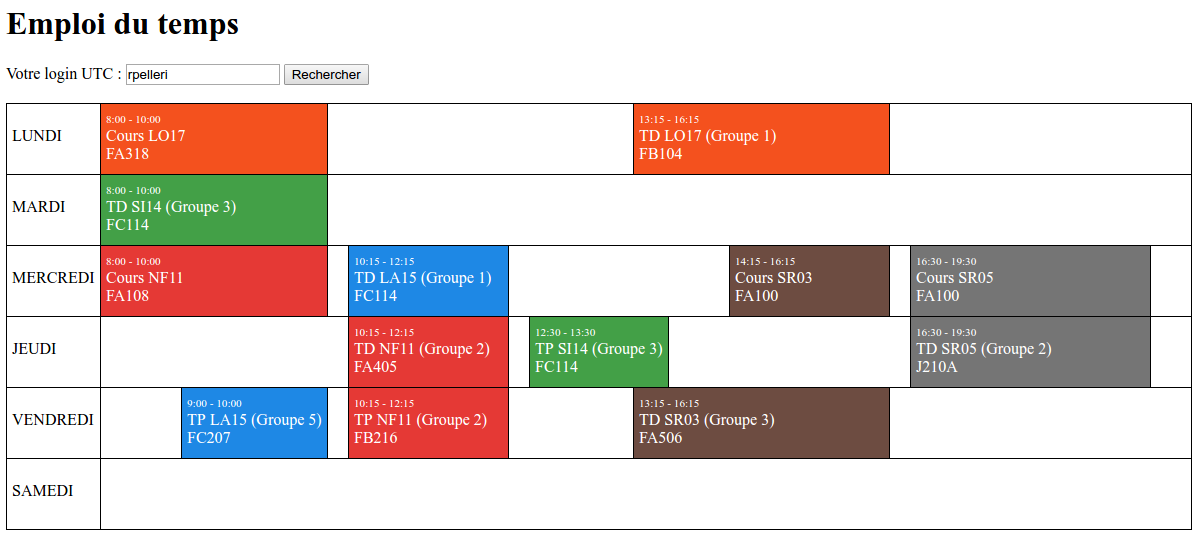
\includegraphics[width=1.00\textwidth]{images/edt.png}
    \caption{Emploi du temps}
\end{figure}
